\section{Related Work}

Given a planar contour, representing the intersection of a plane and a 3D solid object, the task is to generate a path in the domain bounded by the contour.
The nozzle is then instructed to move along the path while extruding material.
The deposited material covers the path with a certain width.
Toolpath generation is an integral part of process planning for 3D printing.
For an overview of the processing pipeline, we refer to the survey by \citeauthor{Livesu2017CGF}.~\cite{Livesu2017CGF} .
For reducing printing time and material cost, sparse infill structures such as triangular and hexagonal patterns have been used to approximate the interior of 3D shapes.
In this paper, we focus on generating toolpath that seamlessly covers the entire 2D contour.
This is sometimes called dense infill~\cite{Livesu2017CGF}.

Toolpath has a direct influence on the printing time, material cost, and mechanical properties of the printed object.
There are a few desirable properties for the toolpath.
First, the path shall be as continuous as possible.
A discontinuous path requires to stop and restart material extrusion. 
For certain material such as TPU, this could lead to material defects~\cite{KUIPERS2019CAD}.
Furthermore, a smooth path is often preferred.
A path with a lot of sharp turns requires to slow down the movement of the nozzle, and this consequently prolongs the printing process.
Second, the path, extended with a certain width, ideally shall cover the bounded region no voids or gaps --  underfilling, and no overlap -- overfilling.
Our method is primarily concerned with this requirement. 

Direction parallel and contour parallel are two basic toolpath strategies.
Direction parallel (or zig-zag) toolpath fills an arbitrarily shaped contour with a set of parallel, equally spaced line segments.
These parallel segments are linked at one of their extremities, to avoid frequent stop and restart.
Contour parallel toolpath typically consists of a set of equally spaced offset contours from the slice boundary.
A strategy to connect the parallel offsets was introduced in~\cite{KUIPERS2019CAD}. This approach however introduces sharp turns.
To reduce the number of sharp turns thereby enable faster motions, \citeauthor{Zhao2016} proposed to use Fermat spiral to cover the contour ~\cite{Zhao2016}.
One of the problems with contour parallel toolpath is that it tends to leave gaps within the slices.
This is due to the fact that the offset contour meets around the medial axis and the remaining space might not match exactly the (constant) deposition width.
To avoid problems with such gaps, hybrid approaches that combine direction and contour parallel are often used~\cite{Mcmains2000DETC,Jin2013adaptive}.
Close to the slice boundary there are a few contour parallel curves, while in the interior there is a zig-zag pattern.
For complex shapes, the entire cross-section could be decomposed into a set of patches, and for each of them, the basic strategies can be applied~\cite{Ding2014,Jin2017JCIM}.
Alternative toolpath patterns, seen also in CNC machining, include space-filling curves~\cite{Cox1994CAD,Griffiths1994,Shaikh2016}.

Our idea to reduce under- and over-filling is to deposit material with a varying width.
This allows the opportunity to locally match the nonuniform space between adjacent paths, and thus to ensure a better coverage of the domain.
Material extraction with a varying width can be realized by changing the extrusion rate or the nozzle travel velocity~\cite{Ertay2018,Kuipers2018}.
However, we note that the range of possible widths is not unlimited.
For instance, printing a width that is tripple the nozzle diameter is challenging.
Our method to reduce underfilling is related to the work by \citeauthor{kao1998optimal}~\cite{kao1998optimal}.
Instead of uniform offsetting, they produced adaptive offsetting toolpaths based on the geometry skeleton. 
Skeleton was also used in~\cite{Jin2017} to construct a skeleton-based path for alleviating under- and over-filling in contour parallel toolpath. 
The adaptive offsetting approach by \citeauthor{kao1998optimal} handles simply geometry where there are no branches in the medial axis.
An extension was proposed by \citeauthor{Ding2016a} to handle complex shapes~\cite{Ding2016a}.
For this purpose, they made use of the medial axis to decompose the slice into a set of simple geometries.
This extension, however, inherits a problem in the original method.
From any point in the geometry skeleton to the boundary, the number of contours is constant.
Since the distance may vary considerably, this strategy leads to a toolpath with widths that may differ by a factor of two or more.
In this paper we propose an adaptive beading strategy to address this problem. 

Besides under- and over-filling, there are a few other robustness issues in toolpath generation, especially concerning thin geometric features.
\todo{Being able to print thin geometrical features can be seen as a a special case of the goal to preventing underfill regions.}
\citeauthor{Moesen2011} proposed a method to make beam compensation more reliable for thin geometric features~\cite{Moesen2011}.
\citeauthor{Behandish2019a} presented a method to characterize local- topological discrepancies due to material under- and over-deposition, and used this information to modify the as-manufactured outcomes~\cite{Behandish2019a}.




% \subsection{Toolpath strategies}
% Simple Zig-Zag toolpathing strategy. \cite{mcmains2000layered}
% Patchwise Zig-Zag toolpathing strategy. \cite{Ding2014}

% Combining concentric toolpaths into continuous extrusion spirals. \cite{Held2009}

% Fractal based toolpaths. \cite{Griffiths1994, mandal2016}

% \subsection{Space filling toolpaths}
% \todo{find other literature which tries to minimize underfilling and overfilling which is not based on a skeletonization.}


% \subsection{Medial axis based toolpaths}
% Adjusted Medial Axis Transform (MAT) structure for only printing the outer wall, rest area to be filled using normal infill. \cite{Moesen2011}
% \Cref{moessen}
% Problem: small grey areas which are too small for the second wall lines.

% Figuring out underfilling and overfilling arteas in concentric fill and using single squigly lines to prevent overfilling. \cite{Jin2017}
% \Cref{jin}

% Using variable width lines to fit a precise amount of lines using the MAT.
% \cite{Ding2016a} apply the method from \cite{kao1998optimal}.
% \Cref{ding}

% \begin{figure}
% \begin{subfigure}{0.45\columnwidth}
% 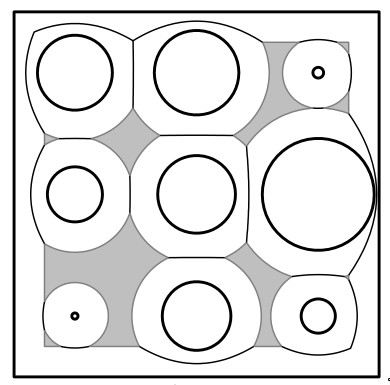
\includegraphics[width=\columnwidth]{sources/related_work/moessen.jpg}
% \caption{\citeauthor{Moesen2011}}
% \label{moessen}
% \end{subfigure}
% \begin{subfigure}{0.45\columnwidth}
% 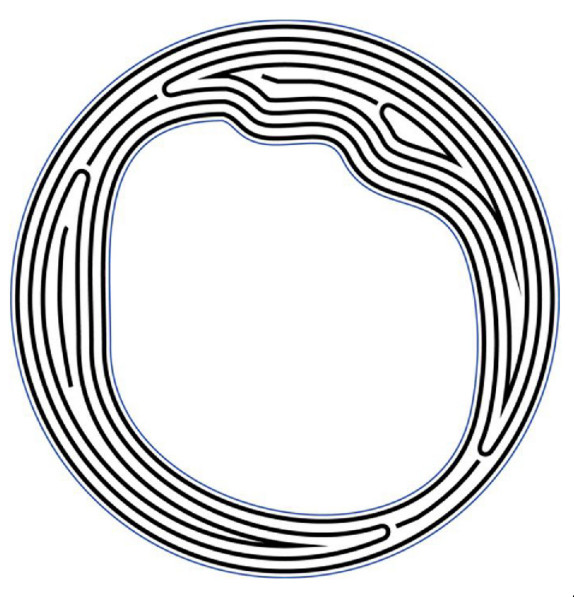
\includegraphics[width=\columnwidth]{sources/related_work/jin.jpg}
% \caption{\citeauthor{Jin2017}}
% \label{jin}
% \end{subfigure}
% \end{figure}

% \begin{figure}
% \centering
% 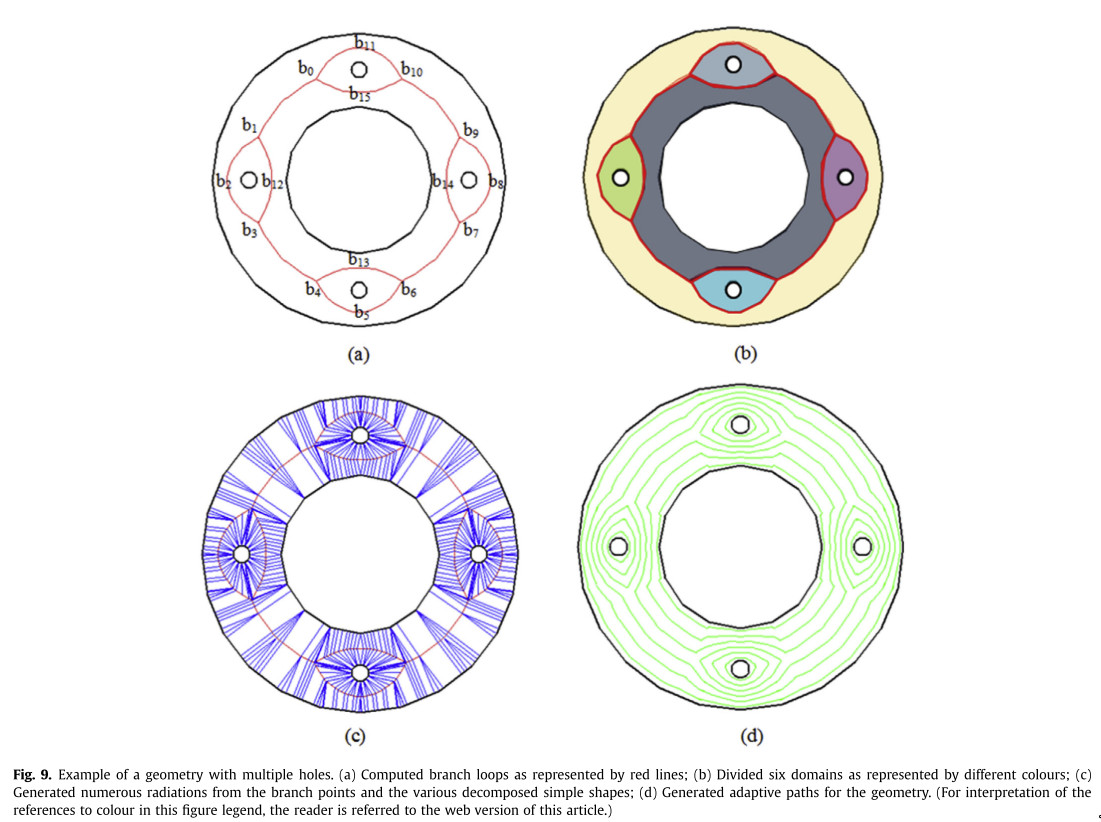
\includegraphics[width=\columnwidth]{sources/related_work/ding.jpg}
% 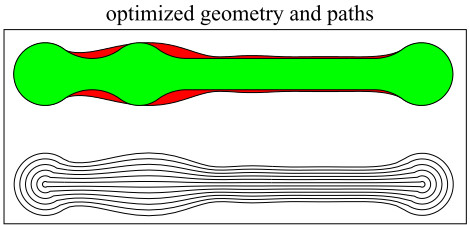
\includegraphics[width=.7\columnwidth]{sources/related_work/kao.jpg}
% \caption{Path planning strategies proposed by Kao (bottom) and employed in FDM by Ding et al (top).}
% \label{ding}
% \end{figure}

% \subsection{Variable extrusion width}

% Changing extrusion rate and temperature to match a given velocity. \cite{Ertay2018}

% Changing velocity in order to change extrusion rate.
% Shortly discussed in \cite{Kuipers2018}.
% \todo{find another reference}